\chapter{Evaluation}

In this chapter we will show some experiment results of our system. We will use various applications which will cover all the aspects of our implementation include thread interleaving synchronization, application instrumentation and system call synchronization. With all the evaluation, we will answer the following questions:

\begin{itemize}
  \item Correctness: Given the same input, can the primary and secondary consistently generate the same output?
  \item Performance: Compare to non-replicated execution, how much overhead is introduced by our system?
  \item Overhead: What do we need to pay for doing replication?
\end{itemize}
% Evaluation factors:
% 1. Lock count & pcnmsg count for schedule part
% 2. Breakdown
% 3. Absolute time

\paragraph{Evaluation Setup} All experiments were run on a server machine with 4 AMD Opteron 6376 Processors (16 cores each, 2.3Ghz), which is 64 cores in total. The total RAM is 128GB. Our Popcorn Linux kernel was installed on Ubuntu 12.04 LTS. We partitioned the hardware resources into half, one for the primary and one for the secondary. Each of them has the full control of their own 32 cores and 64GB RAM. The machine comes with a 1Gbps high speed connection. For benchmarking server applications, we used another server machine in the same rack, connected to the same switch, to act as the benchmark client.

\section{Racey}
We used a variant of racey~\cite{hillstress} to evaluate if our system can work correctly under various concurrent models, in other words, to evaluate the ability of maintaining the same thread-interleaving on all replicas. racey benchmark is a set of concurrent programs which read and write some shared data concurrently with various concurrent models. With a non-deterministic system, all the benchmark will create a different result during each different run. We use racey to validate if we can have the same thread interleaving on primary and secondary, which should lead the same output on both primary and secondary.

\paragraph{racey-guarded} racey-guarded has a global array, it uses pthread to create multiple threads and modify the global array concurrently. The access to the global array is protected by pthread\_mutex\_lock. We tested this one without any modification to the application. With both synchronization algorithms, we are able to create consistent results on the primary and secondary for over 100 consecutive runs.

\paragraph{racey-forkmmap} racey-forkmmap utilizes mmap to create a shared memory area, and uses fork to create multiple processes to read and modify the shared memory area. We 	added \_\_det\_start and \_\_det\_end around each access to the shared memory area. With both synchronization algorithms, we are able to create consistent results on the primary and secondary for over 100 consecutive runs.

\paragraph{racey-tcp} Based on the idea of racey, we developed racey-tcp to stress the determinism for network I/O related tasks. racey-tcp uses pthread to create multiple threads. One thread listens to the socket, whenever a new connection arrives, it puts the connection into a queue, other threads retrieve the connection from the queue, read the data on that connection and write the data into a file. For this benchmark, we wrapped the write system call for writing to the file with \_\_det\_start and \_\_det\_end. With both synchronization algorithms, we are able to create consistent output file on the primary and secondary for over 2000 requests.

\section{PBZip2}
% 1. threading model
% 2. A table of lock and cond var count
% 3. A table of instrumented dettick count
PBZip2~\cite{gilchristparallel} is the parallel version of bzip2. The concurrent model of this application is a typical producer-consumer model, as shown in Figure~\ref{f:pbzip_model}. The FileReader thread reads the content of the file, break the input data into data chunks and put all the chunks into a queue. Worker threads get the data chunks from the queue and do the compression/decompression, after all put the produced data to another queue. The FileWriter will keep getting products from the queue and write them to the final zip file. Multiple pthread\_mutex\_lock and pthread\_cond\_wait functions are applied to provide the mutual exclusion to the access of the queues.

\begin{figure}
\centering
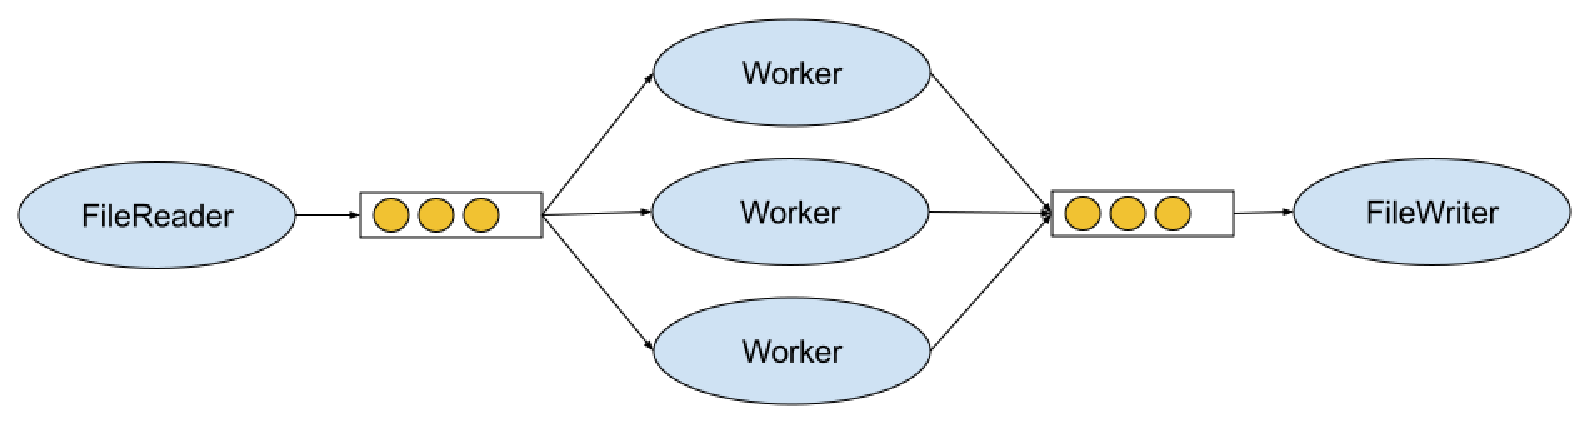
\includegraphics[width=0.8\columnwidth]{figures/pbzip2_model}
\caption{pbzip2 concurrent model}
\label{f:pbzip_model}
\end{figure}

For PBZip2, the time consuming part is the place where it calls the libz2 compression/decompression functions. In this benchmark, we utilized the execution time profiling instrumentation to balance the logical time for the deterministic execution, while for schedule replication nothing is modified. The benchmark is to compress a 177MB file with different thread counts, here we measure the performance with the total execution time reported by pbzip2. Other than that, no manually code modification was applied to the original source code.

Table~\ref{t:pbzip2_syscall} shows the system calls that are used by pbzip2, we only show the system calls that are tracked and synchronized by our system. In pbzip2,  gettimeofday is used for showing the time spent on the whole process, which it is not critical to the output of the application. However pthread\_cond\_timed\_wait also uses gettimeofday to calculate the timeout for the wait time, which is critical to the consistency of the execution.

\begin{table}
 \caption{Tracked system calls used by pbzip2}
\begin{center}
 \begin{tabular}{c | c}
 System Call & Use in the Application\\ \hline
 gettimeofday & Calculate execution time/pthread\_cond\_timed\_wait
 \end{tabular}
\end{center}
\label{t:pbzip2_syscall}
\end{table}

\paragraph{Correctness} For Deterministic Execution, any mismatch of the schedule will lead to different calling sequence of gettimeofday on the primary and secondary, which will result different reported execution time. For Schedule Replication, any mismatch of the schedule will lead the secondary waiting for a wrong schedule event forever. Neither of the case happened during the benchmark, the correctness of the replication thus proven.

\subsection{Results}

Figure~\ref{f:pbzip_b10_performance} shows the execution time of vanilla Linux, Deterministic Execution and Schedule Replication. Both replication modes achieved decent scalability. However, as we can see in Table~\ref{t:pbzip2_overall}, both algorithms' overhead increases with the thread count. One important overhead source for both replication modes comes from the serialization of all the synchronization primitives. With increasing thread count, the downside of breaking the parallelism of accessing those regions becomes more obvious.

For Deterministic Execution, another type of overhead comes from the logical time imbalance. As we mentioned before, the execution profiler takes the average execution time of basicblocks. However the execution time may vary during the actual run, especially for those basic blocks with file I/O, which has non-determinisitc execution time. Although the instrumented pbzip2 showed decent scalbility, the performance still could have been better if we could increase the logical time more precisely.

%different block sizes
\begin{figure}
\centering
\includegraphics[width=0.8\columnwidth]{figures/pbzip2_b10}
\caption{pbzip2 performance}
\label{f:pbzip_b10_performance}
\end{figure}

\begin{table}
\caption{pbzip2 Overall Overhead of Each Replication Mode}
\begin{center}
 \begin{tabular}{c | c | c}
Thread count & Deterministic Execution & Schedule Replication \\ \hline
 2 & 14.27\% & 0.89\% \\ \hline
 4 & 29.47\% & 4.08\% \\ \hline
 8 & 44.77\% & 6.72\% \\ \hline
 16 & 54.44\% & 24.7\% \\ \hline
 24 & 63.39\% & 36.3\% \\ \hline 
 \end{tabular}
\end{center}
\label{t:pbzip2_overall}
\end{table}

\subsection{Message Breakdown}
Figure~\ref{f:pbzip2_msg} shows the number of messages that were used during the benchmark. In all the figures, "Syscall Messages" is the message count for synchronizing system calls, "Network Messages" mean the message count for replicating the network stack, and "Schedule Messages" means the messages for Tick Shepherd in Deterministic Execution, while in Schedule Replication this stands for the messages for logging the execution sequence. This result is expected as we assume that Deterministic Execution doesn't require too much communication between the replicas. Here all the system call messages are for gettimeofday, and most of them are from pthread\_cond\_timed\_wait. In pbzip2, pthread\_cond\_timed\_wait is used by Worker threads to wait for available data chunks. An interesting finding is that for the same benchmark Deterministic Execution invoked less system calls than Schedule Replication. This is because for Deterministic Execution there is a minor logical time imbalance issue, where the FileReader and FilerWriter had more chance to run compare to Worker threads. In this situation, whenever a Worker thread has chance to run, it is very likely to find an available data chunk in the queue, thus no need to call pthread\_cond\_timed\_wait. However for Schedule Replication, the arbitrary thread interleaving causes the Worker threads having more chance waiting on an empty queue, which leads to more invocation to pthread\_cond\_timed\_wait.
\begin{figure}
\centering
\includegraphics[width=1\columnwidth]{figures/pbzip2_msg}
\caption{pbzip2 messages}
\label{f:pbzip2_msg}
\end{figure}

\section{Mongoose Webserver}
% 1. threading model
% 2. A table of lock and cond var count

Mongoose~\cite{mongoose} is a compact multithreaded webserver. The concurrent model is shown in Figure~\ref{f:mongoose_model}. The MasterThread opens a listening socket, uses poll to wait for the incoming connections on the listening socket. Whenever a connection comes, the MasterThread accepts it and put the file descriptor to a queue. WorkerThreads get the connections from the queue and make the response to the clients. Table~\ref{t:mongoose_syscall} shows the system calls that are used by mongoose. The non-deterministic points in mongoose comes from both the thread-interleaving and system call output: diverged thread-interleaving leads to WorkerThreads handling incorrect sockets; diverged system call output leads to incorrect socket state and output value.

We used ApacheBench to stress test mongoose with different file sizes and different mongoose thread counts. For each benchmark set, we used 100 concurrent connections to make 20000 requests in total. For our benchmark on Deterministic Execution, since the file I/O is set to be blocking in mongoose and we do not track file I/O with Tick Shepherd, we manaully added a \dettick\ right before the file I/O system call with an optimal value (only 1 line). Other than that, nothing was changed for mongoose.

\begin{figure}
\centering
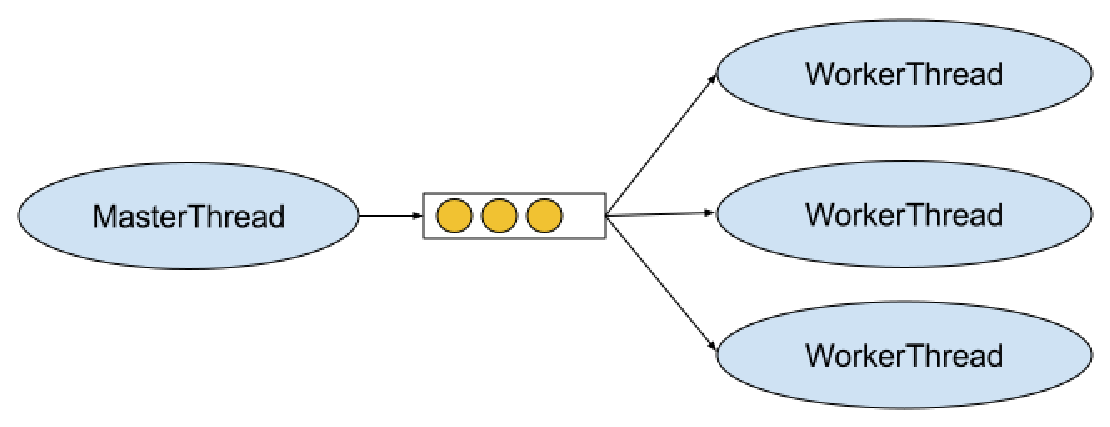
\includegraphics[width=0.6\columnwidth]{figures/mongoose_model}
\caption{mongoose concurrent model}
\label{f:mongoose_model}
\end{figure}

%Given mongoose's concurrent model, we can see that different file size will affect the frequency of acquiring locks. In this way we can figure out how will two algorithm perform under different lock acquisition load. Also, different thread counts can reflect the scalability of our system.
%cite ab

\begin{table}
\caption{Tracked system calls used by mongoose}
\begin{center}
 \begin{tabular}{c | c}
System Call & Use in the Application\\ \hline
 time & Generate HTTP header  \\ \hline
 poll & Wait for accept, read and write
 \end{tabular}
\end{center}
\label{t:mongoose_syscall}
\end{table}

\paragraph{Correctness} For both replication mode, any mismatch will lead to either different thread handling different socket, or divergence in the HTTP responses. Neither of the case happened during the benchmark, the correctness of the replication thus proven.

\subsection{Results}
\begin{figure}
\centering
\includegraphics[width=0.7\columnwidth]{figures/mg_throughput_50k}
\caption{mongoose performance for 50KB file requests}
\label{f:mg_50k}
\end{figure}
\begin{figure}
\centering
\includegraphics[width=0.7\columnwidth]{figures/mg_throughput_100k}
\caption{mongoose performance for 100KB file requests}
\label{f:mg_100k}
\end{figure}
\begin{figure}
\centering
\includegraphics[width=0.7\columnwidth]{figures/mg_throughput_200k}
\caption{mongoose performance for 200KB file requests}
\label{f:mg_200k}
\end{figure}

\begin{table}
\caption{Mongoose Overall Overhead of Each Replication Mode}
\begin{center}
 \begin{tabular}{c | c | c}
Thread Count & Deterministic Execution & Schedule Replication \\ \hline
 4 & 25.22\% & 1.35\% \\ \hline
 8 & 15.72\% & 0.27\% \\ \hline
 16 & 9.82\% & 0.23\% \\ \hline
 \end{tabular}
\end{center}
\label{t:mongoose_overall}
\end{table}

Figure ~\ref{f:mg_50k}, ~\ref{f:mg_100k} and ~\ref{f:mg_200k} show the performance under different workload, and Table ~\ref{t:mongoose_overall} shows the overall overhead of each replication mode. Deterministic Execution's overhead becomes lower as the thread count goes up, but still higher than Schedule Replication. This is due to blocking socket write and file I/O  operations. Because the time spent inside those blocking I/O varies all the time, our manually inserted \dettick\ couldn't precisely increase the logical time for every call, as a result we had to suffer the performance loss from logical time imbalance. In the meanwhile, Schedule Replication showed near zero overhead compare to the baseline.

Unlike pbzip where the overhead becomes higher when the thread count increases, mongoose's overhead decreases with more number of threads. This is because monoogse only has two condition variables and one mutex lock, the side effect of serializating pthread primitives is minimal and the performance thus can scale.

\subsection{Message Breakdown}
Figure~\ref{f:mg_msg_50k}, Figure~\ref{f:mg_msg_100k} and Figure~\ref{f:mg_msg_200k} show the breakdown of overall messages for each benchmark set. The notation is the same as the previous section. Where "Schedule Messages" means the messages for Tick Shepherd in Deterministic Execution, a in Schedule Replication this stands for the messages for logging the execution sequence.

Actually, we need much more messages for deterministic execution, which contradicts the assumption we made for Deterministic Execution. In mongoose, socket write and file I/O are blocking operations, and bigger network payload leads to more socket calls, thus we need more messages for the Tick Shepherd to synchronize the tick bumps. However for Schedule Replication, since the messages for scheduling only depends on the number of synchronization primitives, which totally depends on the number of requests (not the size), as a result, across all the benchmarks, the number of schedule messages for Schedule Replication show a near constant value across all the benchmarks.

\begin{figure}
\centering
\includegraphics[width=0.7\columnwidth]{figures/mg_msg_50k}
\caption{mongoose messages for 50KB file requests}
\label{f:mg_msg_50k}
\end{figure}
\begin{figure}
\centering
\includegraphics[width=0.7\columnwidth]{figures/mg_msg_100KB}
\caption{mongoose messages for 100KB file requests}
\label{f:mg_msg_100k}
\end{figure}
\begin{figure}
\centering
\includegraphics[width=0.7\columnwidth]{figures/mg_msg_200KB}
\caption{mongoose messages for 200KB file requests}
\label{f:mg_msg_200k}
\end{figure}
\section{Nginx Webserver}

Nginx~\cite{reese2008nginx} is a sophisticated webserver with multiple threading modes. In this benchmark we used the threadpool setup~\cite{nginxthreadpool} for our benchmark. As shown in Figure~\ref{f:nginx_model}, in this threading mode, the additional threads are only for doing file I/O operations. The MasterThread waits on the listening socket, whenever a file request is coming, it hands over the request into a queue. WorkerThreads get notified whenever a new request is coming and try to retrieve one task from the queue. Whenever the content of the requested file is loaded into memory by a WorkerThread, a handle will be put into another queue and the MasterThread will get notified. In the end, the MasterThread will retrieve the handle and send the content of the file back to the client. 

Table ~\ref{t:nginx_syscall} shows all the tracked system calls used by Nginx. All of the I/O operations are asynchronous and heavily relies on epoll mechanism. 

\begin{figure}
\centering
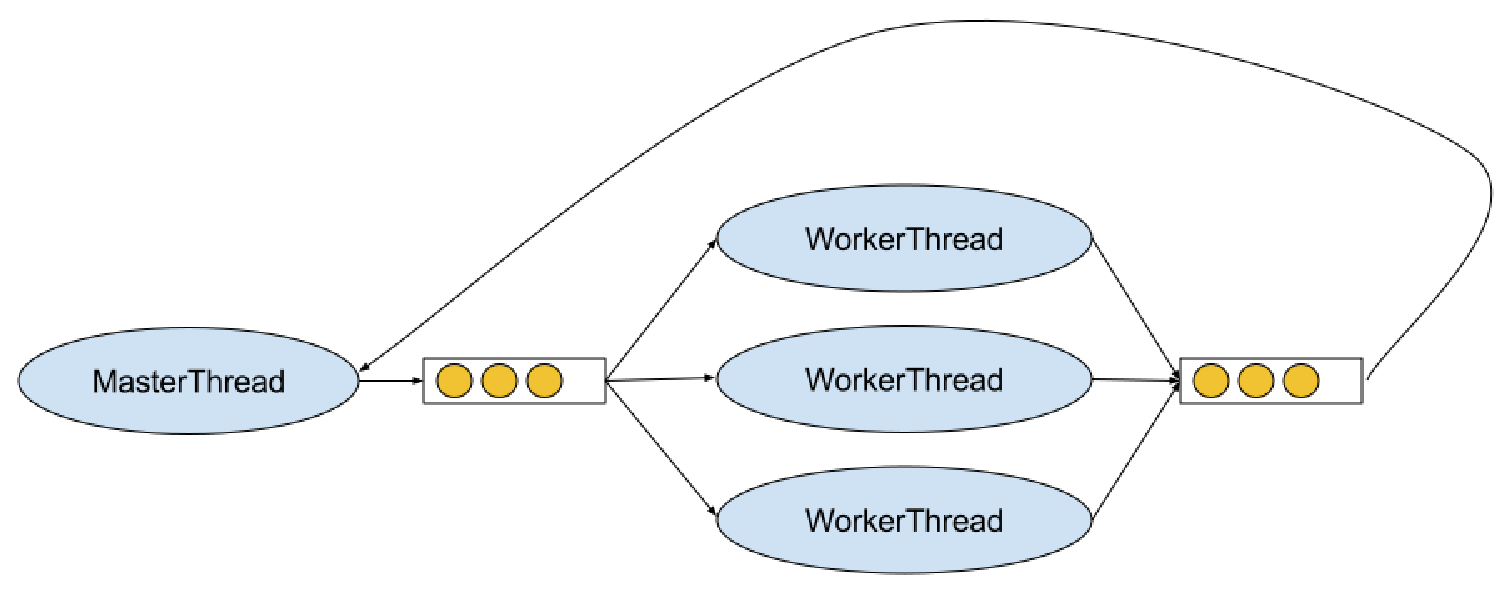
\includegraphics[width=0.8\columnwidth]{figures/nginx_model}
\caption{Nginx thread pool model}
\label{f:nginx_model}
\end{figure}

The same as mongoose, we used ApacheBench to stress test the server with different file sizes and different mongoose thread counts. For each benchmark set, we used 100 concurrent connections to make 20000 requests in total.

Nginx has multiple explicit atomic operations that might lead to non-deterministic results, here we applied \detstart\ and \detend\ around those operations to maintain the total order of those operations. Another non-deterministic part in Nginx is that it uses eventfd to communicate among threads. As we mentioned before, all inter-thread communication need to be deterministic on all the replicas, as a result, we applied \detstart\ and \detend\ around the read and write operations of eventfd to synchronize the total order of those operations. Other than that, no further modification were applied. In total, we added around 60 LOC to the original code.
%cite event fd here

\begin{table}
\caption{Tracked system calls used by nginx}
\begin{center}
 \begin{tabular}{c | c }
System Call & Use in the Application\\ \hline
 gettimeofday & Generate HTTP header\\ \hline
 epoll\_wait & Wait for accept, read and write
 \end{tabular}
\end{center}
\label{t:nginx_syscall}
\end{table}

\paragraph{Correctness} Similar to mongoose, any mismatch will lead to either different thread handling different socket, or divergence in the HTTP responses. Neither of the case happened during the benchmark, the correctness of the replication thus proven.

\subsection{Results}
\begin{figure}
\centering
\includegraphics[width=0.8\columnwidth]{figures/ng_throughput_50k}
\caption{nginx performance for 50KB file requests}
\label{f:ng_50k}
\end{figure}
\begin{figure}
\centering
\includegraphics[width=0.8\columnwidth]{figures/ng_throughput_100k}
\caption{nginx performance for 100KB file requests}
\label{f:ng_100k}
\end{figure}
\begin{figure}
\centering
\includegraphics[width=0.8\columnwidth]{figures/ng_throughput_200k}
\caption{nginx performance for 200KB file requests}
\label{f:ng_200k}
\end{figure}

\begin{table}
\caption{Nginx Overall Overhead of Each Replication Mode}
\begin{center}
 \begin{tabular}{c | c | c}
Thread Count & Deterministic Execution & Schedule Replication \\ \hline
 4 & 3\% & 1.07\% \\ \hline
 8 & 1.62\% & 1.96\% \\ \hline
 16 & 1.6\% & 1.31\% \\ \hline
 \end{tabular}
\end{center}
\label{t:nginx_overall}
\end{table}

The reason we see the result is not scaling (even for Linux) is because this threading mode for Nginx is only for concurrent file I/O. During our benchmark, we've already achieved the best of our filesystem even with lower thread counts, although all the threads were loaded, putting more threads won't increase the performance too much. However, the purpose of the benchmark is to show that how will different thread counts affecting our system's overhead (comparing to baseline), a non-scaling result still makes sense here.

Unlike mongoose, the result of Nginx showed both replication modes can achieve very small overhead. When we take a step back to deterministic execution, the major performance hurdle is the logical time imbalance, which happens when there are some time consuming code sections. However, since nginx fully utilizes asynchronous file and network I/O, everything is super fast. In the context of deterministic execution, we can say in Nginx there is no significant time consuming part that will cause logical time imbalance. Therefore Deterministic Execution can perform its best.

%On the other hand, the massive amount of messages used by Schedule Replication has put a more obvious overhead to the execution. That is why we are able to see Deterministic Execution can perform better.

\subsection{Message Breakdown}
\begin{figure}
\centering
\includegraphics[width=0.8\columnwidth]{figures/ng_msg_50KB}
\caption{nginx messages for 50KB file requests}
\label{f:ng_msg_50k}
\end{figure}
\begin{figure}
\centering
\includegraphics[width=0.8\columnwidth]{figures/ng_msg_100KB}
\caption{nginx messages for 100KB file requests}
\label{f:ng_msg_100k}
\end{figure}
\begin{figure}
\centering
\includegraphics[width=0.8\columnwidth]{figures/ng_msg_200KB}
\caption{nginx messages for 200KB file requests}
\label{f:ng_msg_200k}
\end{figure}
%The message breakdown has proved the analysis we made. Without any logical time imbalance, messaging and serilization are the only overhead sources for the system for Deterministic Execution.
Figure ~\ref{f:ng_50k}, figure ~\ref{f:ng_100k} and figure ~\ref{f:ng_100k} show the message break for our benchmark. As mention in the beginning of this section, Nginx needs more \detstart\ and \detend\ other than pthread primitives, so Schedule Replication uses way more messages than Deterministic Execution. Another interesting fact is that since asynchronous I/O operations are really fast in Nginx, in Deterministic Execution, the Tick Shepherd barely made a tick bump, which is also a reason that Deterministic Execution could perform much better than it was in mongoose. While in mongoose, almost every blocking I/O had at least one tick bump.

%\section{Redis Database Server}
%Redis is an in-memory database server. It uses a single thread to process requests, but it dynamically creates new threads to write the in-memory data to the disk. This benchmark is perfect for stressing the flexibility of dealing with dynamically spawned threads.

%For the performance test we used the redis-benchmark tool, we used the default benchmark parameter which will test all the operations. Each operation is tested for 10000 requests. We also have different number of concurrent clients to stress the server with different frequency of requests. We ran each setup for 5 times and took the average of the numbers.

%Redis uses an alternative memory allocator jemalloc, which contains some internal locks to ensure mutual exclusion for concurrent memory allocation. As mentioned in Section~\ref{sec:elision}, those lock acquisitions doesn't affect the output at all, so we modified the jemalloc's source code, to skip the synchronizations for those locks. Other than that, no further modification was made to the application.

%\subsection{Results}
%Figure~\ref{f:redis_2}, figure~\ref{f:redis_16} and figure~\ref{f:redis_64} show the  performance of redis with 2, 16 and 64 concurrent clients. Table~\ref{t:redis_overall} shows the overall overhead of each replication mode.

%The configuration was set to save the data every 10000 requests, which means for each benchmark of each operation, we will have one write back to the disk.

%\begin{figure}
%\centering
%\includegraphics[width=0.8\columnwidth]{figures/redis_2}
%\caption{redis benchmark with 10000 requests and 2 clients}
%\label{f:redis_2}
%\end{figure}

%\begin{figure}
%\centering
%\includegraphics[width=0.8\columnwidth]{figures/redis_16}
%\caption{redis benchmark with 10000 requests and 16 clients}
%\label{f:redis_16}
%\end{figure}

%\begin{figure}
%\centering
%\includegraphics[width=0.8\columnwidth]{figures/redis_64}
%\caption{redis benchmark with 10000 requests and 64 clients}
%\label{f:redis_64}
%\end{figure}

%\begin{table}
%\caption{Redis Overall Overhead of Each Replication Mode}
%\begin{center}
% \begin{tabular}{c | c | c}
%Client count & Deterministic Execution & Schedule Replication \\ \hline
% 2 & 30.38\% & 11.93\% \\ \hline
% 16 & 41.05\% & 26.94\% \\ \hline
% 64 & 39.66\% & 26.48\% \\ \hline
% \end{tabular}
%\end{center}
%\label{t:redis_overall}
%\end{table}

%\subsection{Message Breakdown}

\section{Discussion}
The selected benchmarks were used to stress different aspects of this project. Although there are still some optimizations to go, we still achieved decent overhead for different types of concurrent models and different application types. Here we will discuss some interesting issues during the benchmark and some findings from the results.

\subsection{Benchmark for Nginx's Multi-process Mode}
So far for all the marco benchmarks, we only showed benchmarks for multi-threaded applications. However our system also supports replication for multi-process applications (as we showed for racey microbenchmark). Nginx supports multi-worker mode, which spawns multiple worker processes, all of the worker processes wait on the listening socket together. Nginx implements the accept\_mutex ~\cite{nginxscalability}, which is lock across processes, to ensure an incoming request only wakes up one waiting worker. In order to figure out whether our replication works for this concurrent model or not, we manually instrumented the accept\_mutex acquisition with \detstart\ and \detend\ . During the benchmark, both primary and secondary were able to end up with the same state all the time. However no matter how many workers we put, it was always only one worker handling all the request. This is due to a relatively low workload we used in our benchmark. However, because of the limitation of our network card (1Gbps), we couldn't apply heavier workload to saturate the worker. With Nginx's design, the accept\_mutex mechanism will not pass the request to another worker if the current worker is not saturated. Which is the reason we only saw one worker handling all the requests.

Unlike the non-scaling result with the threadpool mode, where all the threads were fully loaded, the unbalanced workload in multi-worker mode seems not making any sense. As a result we didn't include the result in this chapter.

\subsection{Deterministic Execution's Dilemma}
For deterministic execution, a type of overhead comes from the calculation of the token (finding the task with minimal logical time). Current implementation requires O(N) time to decide which task should execute on next \detstart\ , where N is the number of threads. Every logical time update comes with such a computation process, more threads lead to more computation time.  As we can see from all the benchmarks, deterministic system always leads to a higher overhead when thread count increases. In a previous discussion ~\cite{bergan2011deterministic}, it is pointed out that all the existing deterministic systems, regardless of what type of deterministic algorithm (lockstep or wait for turn), this kind of global communication is inevitable. This also implies that deterministic might not be practical for highly concurrent application with highly intensive inter-thread communications (synchronization primitives). Webservers like mongoose and nginx have very simple inter-thread communication , so that we achieved decent overhead during the benchmark. But for more complicated applications with more different types of locks, we might face severe performance overhead.

\subsection{Which Replication Mode Should I Use?}
From all the benchmarks, we saw that some are better for Deterministic Execution and some are better for Schedule Replication. Figure~\ref{f:trade_off} shows the basic idea of what kind of price we are paying for different replication modes. For Deterministic Execution, if we are able to precisely balance the logical time, or there is no logical time imbalance problem (like Nginx), it is the choice. For Schedule Replication, since on Popcorn Linux, the cost of sending a message is under 2 microseconds, despite the huge amount of messages that Schedule Replication needs, the overall overhead from messaging can nearly be ignored. As long as the cost of sending messages keeps low, Schedule Replication is always the better choice.

\begin{figure}
\centering
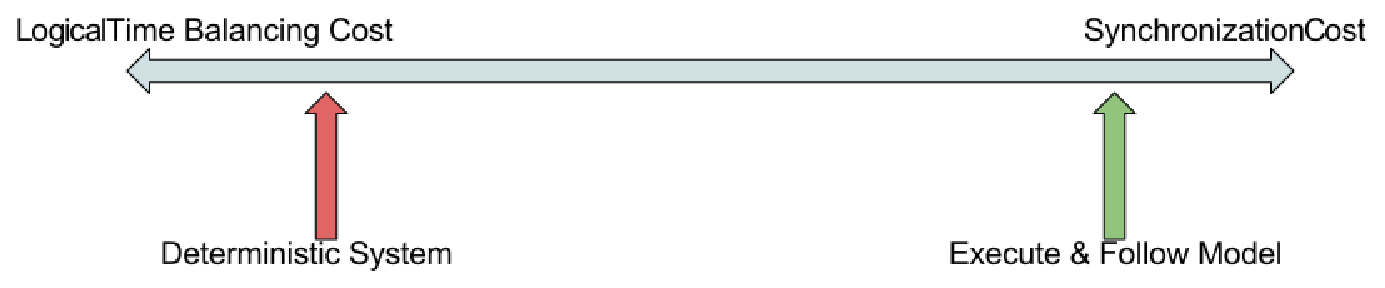
\includegraphics[width=1\columnwidth]{figures/tradeoff}
\caption{The tradeoff of two replication modes}
\label{f:trade_off}
\end{figure}